\documentclass{article}
\usepackage[margin = .7in]{geometry}
\usepackage[dvipdfmx]{graphicx}
\usepackage{listings}
\usepackage{amsmath}
\usepackage{bm}
\lstset{%
  language={python},
  basicstyle={\small},%
  identifierstyle={\small},%
  commentstyle={\small\itshape},%
  keywordstyle={\small\bfseries},%
  ndkeywordstyle={\small},%
  stringstyle={\small\ttfamily},
  frame={tb},
  breaklines=true,
  columns=[l]{fullflexible},%
  numbers=left,%
  xrightmargin=0zw,%
  xleftmargin=3zw,%
  numberstyle={\scriptsize},%
  stepnumber=1,
  numbersep=1zw,%
  lineskip=-0.5ex%
}

\begin{document}
\title{Econometrics 2 2017 \\ 
Problem set 1}
\author{Kei Ikegami (150012)}
\maketitle

\section{Problem 1}
\subsection{(a)}
Let $\epsilon = y - \alpha - x^{'}\beta$, where $\alpha = E[y] - E[x^{'}]\beta$ and $\beta = \Sigma^{-1}\delta$, then I show $E[\epsilon] = 0$  and $E[\epsilon x] = 0$. 
\begin{align*}
	E[\epsilon] &= E[y - E[y] + E[x^{'}]\beta - x^{'}\beta] = E[(y - E[y]) - (x^{'} - E[x^{'}])\beta] = (E[y] - E[y]) - (E[x^{'}] - E[x^{'}])\beta = 0\\[8pt]
	E[\epsilon x] &= E[x\epsilon] = E[x(y - E[y] + E[x^{'}]\beta - x^{'}\beta)] = E[x(y - E[y]) - x(x^{'} - E[x^{'}])\beta]\\[8pt]
	&= E[(x - E[x])(y - E[y]) + E[x](y - E[y]) - (x - E[x])(x^{'} - E[x^{'}])\beta - E[x](x^{'} - E[x^{'}])\beta]\\[8pt]
	&= \delta - E[(x - E[x])(x^{'} - E[x^{'}])]\Sigma^{-1}\delta = \delta - \delta = 0
\end{align*}
So now I get the result.

\subsection{(b)}
This transformation is useful.
\begin{align*}
	E[(y - a - x^{'}b)^2] = E[(y - E[y])^2] + 2E[(y- E[y])(E[y] - (a + x^{'}b))] + E[(E[y] - (a + x^{'}b))^2]
\end{align*}
Then I get the FOC by differentiating by $a$ as follows.
\begin{align*}
	E[-2(y - E[y])] + E[-2(E[y] - (a + x^{'}b))] = 0\ \Rightarrow \ a = E[y] -E[x^{'}]b
\end{align*}
Next, after inserting the above relationship to the original, I get the FOC by differentiating by $b$ as follows.
\begin{align*}
	-2E[(y - E[y])(x^{'} - E[x^{'}])]^{'} + 2E[(x^{'} - E[x^{'}])^{'}(x^{'} - E[x^{'}])b] = 0\ \Leftrightarrow \ b = \Sigma^{-1}\delta
\end{align*}
And the second derivative by $b$ is $2 \Sigma$, which is positive semi definite, then the second order condition for minimization is fulfilled. Thus I show $\alpha, \beta$ in (a) solves this minimization problem.

Then I show the second part. First I show the important property of the conditional expectation. If $y = E[y|x] + \epsilon$, then $E[\epsilon | x] = E[y - E[y|x] |x] = 0$ and for any function $h(x)$, $E[h(x) \epsilon] = E[E[h(x)\epsilon | x]] = E[h(x)E[\epsilon | x]] = 0$. Using this second property can easily prove the argument.
\begin{align*}
	E[(y - a - x^{'}b)^2] &= E[(y- E[y|x] + E[y|x] -a -x^{'}b)^2] \\[8pt]
	&= E[(y- E[y|x])^2] + 2E[(y - E[y])(E[y|x] -a-x^{'}b)] + E[(E[y|x] - a-x^{'}b)^2]\\[8pt]
	&= E[(y- E[y|x])^2] + E[(E[y|x] - a-x^{'}b)^2]
\end{align*}
The second term in the first line vanishes since $E[(y - E[y])(E[y|x] -a-x^{'}b)] = E[\epsilon(E[y|x] -a-x^{'}b)] = 0$. This is because $E[y|x] -a-x^{'}b$ is just a function of $x$.

\subsection{(c)}
In the real econometric analysis, the relationship $E[\epsilon x] = 0$ is just an assumption. And that the correlation between the regressor and the error is zero needs the situation where all relevant variables are in the regression model, but this is unrealistic because certainly many unobservable variables exist. We can use IV for solving such a situation and get the consistent estimator of the coefficient of interesting variables.

\subsection{(d)}
(b) says that the predicted value by using OLS estimator is the best linear approximate of the conditional mean of the dependent variable even if the form is not linear among the support, when we use squared loss function. This clearly argue the statement.

\subsection{(e)}
houti

\section{Problem 2}
\subsection{(a)}
\begin{align*}
	Cov(Az_i, \epsilon_i) = E[(Az_i - E[Az_i])(\epsilon_i - E[\epsilon_i])] = A E[(z_i - E[z_i])(\epsilon_i - E[\epsilon_i])] = 0
\end{align*}
Therefore $Az_i$ does not correlate with $\epsilon_i$. And clearly the correlation exist between $Az_i$ and $x_i$. Thus $Az_i$ is a valid IV for $x_i$. And $rank(E[Az_i x_i^{'}]) = K$ allows it to have inverse matrix, so IV estimator can be constructed.

\subsection{(b)}
Multiplying $Az_i$ to the first model by left.
\begin{align*}
	Az_iy_i = Az_ix_i^{'}\beta + Az_i\epsilon_i
\end{align*}
Sum up the model by individuals. And divide by $n$.
\begin{align*}
	\sum_{i = 1}^n Az_iy_i = (\sum_{i = 1}^n Az_ix_i^{'})\beta + \sum_{i=1}^nAz_i\epsilon_i \ \Leftrightarrow\ \left(\frac{1}{n}\sum_{i = 1}^n Az_iy_i\right) = \left(\frac{1}{n}\sum_{i = 1}^n Az_ix_i^{'}\right)\beta + \left( \frac{1}{n}\sum_{i=1}^nAz_i\epsilon_i \right)
\end{align*}
Consider the moment condition $E[Az_i\epsilon_i] = 0$. And we have the assumption that $rank(E[Az_i x_i^{'}]) = K$, so the sample analogue of this moment can be inversed. Then I have the IV estimator as the method of moment estimator as follows.
\begin{align*}
	\hat{\beta_A} = \left(\frac{1}{n}\sum_{i = 1}^n Az_ix_i^{'}\right)^{-1} \left(\frac{1}{n}\sum_{i = 1}^n Az_iy_i\right)
\end{align*}

\subsection{(c)}
Using the matrix $A$, I can write the sample moment condition as follows.
\begin{align*}
	\frac{1}{n}\sum_{i = 1}^n \left(\sum_{i = 1}^n x_i z_i^{'}\right)\left(\sum_{i = 1}^n z_i z_i^{'}\right)^{-1} z_i (y_i - x_i^{'}b) = 0
\end{align*}
And I use the following matrix notation to make it easy to see, $\sum_{i = 1}^n x_i z_i^{'} = X^{'}Z$ and $\sum_{i = 1}^n z_i z_i^{'} = Z^{'}Z$. Then the condition leads to the IV estimator.
\begin{align*}
	&\frac{1}{n}\sum_{i = 1}^n \left(X^{'}Z\right)\left(Z^{'}Z\right)^{-1} z_i (y_i - x_i^{'}b) = 0\\[8pt]
	\quad \Leftrightarrow \quad&\sum_{i=1}^n \left(X^{'}Z\right)\left(Z^{'}Z\right)^{-1} z_i y_i = \sum_{i=1}^n \left(X^{'}Z\right)\left(Z^{'}Z\right)^{-1}z_i x_i^{'}b\\[8pt]
	\quad \Leftrightarrow \quad& \left(X^{'}Z\right)\left(Z^{'}Z\right)^{-1}\left(Z^{'}y\right) = \left(X^{'}Z\right)\left(Z^{'}Z\right)^{-1}\left(Z^{'}X\right)b\\[8pt]
	\quad \Leftrightarrow \quad&b = (X^{'}P_ZX)^{-1}X^{'}P_Z y
\end{align*}

\subsection{(d)}
Using matrix notations lead to the result. Note that $Z^{'}X$ has its inverse matrix because $L = K$.
\begin{align*}
	\hat{\beta_A} = (AZ^{'}X)^{-1}AZ^{'}y = (Z^{'}X)^{-1}A^{-1}AZ^{'}y = (Z^{'}X)^{-1}Z^{'}y
\end{align*}
The last term shows it does not depend on $A$.

\section{Problem 3}
I show the result of the regression.
\begin{figure}[h]
    \centering
    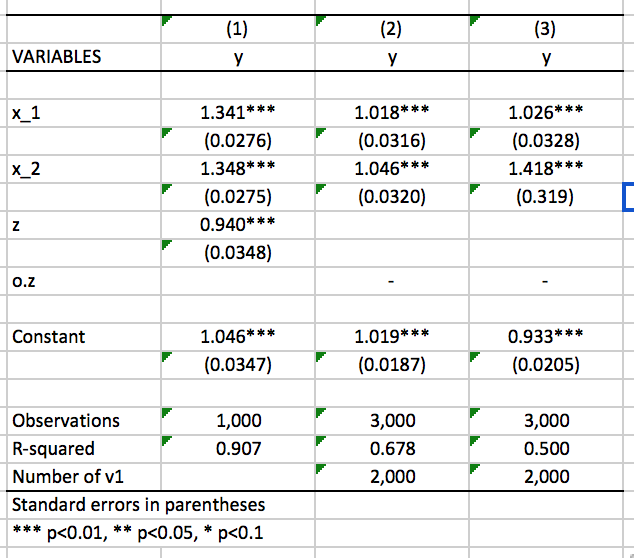
\includegraphics[width=10cm]{3.png}
    \caption{Results of the three regressions}
\end{figure}
Column 1 is the result of the first type of regression, which I use just a one year data and OLS. Column 2 is the second one, which I use all the data and fixed effect estimator. Column 3 is the third one, which I use different data in that $x_{2it} = \alpha_i + 0.1u_{2it}$.
\subsection{(a)}
I use Python in this problem for convenience.

\subsection{(b)}
Constant term and the coefficient of $z_i$ is consistently estimated in this case and the coefficients of $x_{1it}, x_{2it}$ is biased. This is because the first two components do not correlate with the error term while the last two correlates through $\alpha_i$. I see the coefficients of the last two is positively biased, in other words they are bigger than true value $1$. And this is caused by the positive correlations with error term.

\subsection{(c)}
This is done in the first table.

\subsection{(d)}
In this regression, while the estimate of the coefficient of $x_{1it}$ seems to be correct, the coefficient of $x_{2it}$ is positively biased and furthermore has a large standard error as in the first table.

\subsection{(e)}
think

\section{Problem 4}
\subsection{(a)}
The model tells us that
\begin{align*}
	Y_1 = X\beta_1 + E_1\\
	Y_2 = X\beta_2 + E_2
\end{align*}
Therefore it is clear that all in one matrix formulation is the mentioned form.

\subsection{(b)}
$\sigma_{ab}$ denotes the covariance between $\epsilon_{i,a}$ and $\epsilon_{i, b}$. Note that the errors of different individuals do not correlate. The matrix $\Sigma$ is
\begin{align*}
\Sigma = \begin{pmatrix}
\sigma_{11} & \sigma_{12}\\
\sigma_{21} & \sigma_{22}
\end{pmatrix}
\end{align*}

 Let $E$ be the joint errors. Therefore the variance covariance matrix in this model is as follows.
\begin{align*}
	Var\left(E \right) = \begin{pmatrix}\sigma_{11}& 0& \cdots& 0&\sigma_{12}&0 &\cdots & 0\\
	\vdots&&&\vdots&\vdots&&&\vdots\\
	0&0&\cdots&\sigma_{11}&0&0&\cdots&\sigma_{12}\\
	\sigma_{21}& 0& \cdots& 0&\sigma_{22}&0 &\cdots & 0\\
	\vdots&&&\vdots&\vdots&&&\vdots\\
	0&0&\cdots&\sigma_{21}&0&0&\cdots&\sigma_{22}
	\end{pmatrix}
	=\Sigma \otimes I_N
\end{align*}

\subsection{(c)}
By the definition of GLS estimator, I get in this case as follows.
\begin{align*}
	\beta_{GLS} = \left(\left(\begin{array}{cc} X & 0 \\ 0 & X \end{array}\right)^{'} \left(\Sigma \otimes I_N \right)^{-1} \left(\begin{array}{cc} X & 0 \\ 0 & X \end{array}\right)\right)^{-1} \left(\begin{array}{cc} X & 0 \\ 0 & X \end{array}\right)^{'} \left(\Sigma \otimes I_N \right)^{-1} Y
\end{align*}
when $Y = \left(\begin{array}{cc} Y_1\\Y_2 \end{array}\right)$

\subsection{(d)}
By (c)
\begin{align*}
	\beta_{GLS} &= \left(\left(\begin{array}{cc} X^{'} & 0 \\ 0 & X^{'} \end{array}\right) \left(\Sigma^{-1} \otimes I_N \right) \left(\begin{array}{cc} X & 0 \\ 0 & X \end{array}\right)\right)^{-1} \left(\begin{array}{cc} X^{'} & 0 \\ 0 & X^{'} \end{array}\right) \left(\Sigma^{-1} \otimes I_N \right) Y\\[8pt]
	&= \left(\left(\begin{array}{cc} X^{'} & 0 \\ 0 & X^{'} \end{array}\right) \left(\begin{array}{cc} \sigma_{22}I_N & -\sigma_{12}I_N \\ -\sigma_{21} I_N & \sigma_{11} I_N \end{array}\right) \left(\begin{array}{cc} X & 0 \\ 0 & X \end{array}\right)\right)^{-1} \left(\begin{array}{cc} X^{'} & 0 \\ 0 & X^{'} \end{array}\right) \left(\begin{array}{cc} \sigma_{22}I_N & -\sigma_{12}I_N \\ -\sigma_{21} I_N & \sigma_{11} I_N \end{array}\right) Y\\[8pt]
	&= \left( \begin{array}{cc} \sigma_{22}X^{'}X & -\sigma_{12} X^{'}X \\ -\sigma_{21}X^{'}X & \sigma_{11}X^{'}X \end{array} \right)^{-1} \left( \begin{array}{cc} \sigma_{22}X^{'} & -\sigma_{12} X^{'} \\ -\sigma_{21}X^{'} & \sigma_{11}X^{'} \end{array} \right) y\\[8pt]
	&= \left(\left( \begin{array}{cc} \sigma_{22} & -\sigma_{12} \\ -\sigma_{21} & \sigma_{11} \end{array} \right) \otimes X^{'}X\right)^{-1} \left(\left( \begin{array}{cc} \sigma_{22} & -\sigma_{12} \\ -\sigma_{21} & \sigma_{11} \end{array} \right) \otimes X^{'} \right) y\\[8pt]
	&= \left( I_2 \otimes (X^{'}X)^{-1}X^{'} \right) y\\[8pt]
	&= \left( \begin{array}{cc} (X^{'}X)^{-1}X^{'} & 0 \\ 0 & (X^{'}X)^{-1}X^{'} \end{array} \right) \left( \begin{array}{cc} Y_1\\Y_2 \end{array}\right)\\[8pt]
	&= \left( \begin{array}{cc} (X^{'}X)^{-1}X^{'}Y_1 \\ (X^{'}X)^{-1}X^{'}Y_2 \end{array}\right)
\end{align*}
The second equality is from $\Sigma^{-1} = \frac{1}{\sigma_{11}\sigma_{22} - \sigma_{12}^2}\left( \begin{array}{cc} \sigma_{22} & -\sigma_{12} \\ -\sigma_{21} & \sigma_{11} \end{array} \right)$. By the above I get the result.


\section{Problem 5}
\subsection{(a)}
In this case, $\Sigma = \left( \begin{array}{ccc} \sigma_{11}&\cdots&\sigma_{1T}\\ \vdots&&\vdots\\ \sigma_{1T}&\cdots&\sigma_{TT} \end{array} \right)$, where $\sigma_{tt^{'}} = E[\epsilon_{it} \epsilon_{it^{'}} | x_{it}, z_{it^{'}}]$. Using this notations,
\begin{align*}
	Var(E | X) = I_N \otimes \Sigma
\end{align*}

\subsection{(b)}
\begin{align*}
	M &= I_{NT} - \left( I_N \otimes \iota_T \right) \left( \left( I_N \otimes \iota_T \right)^{'} \left( I_N \otimes \iota_T \right) \right)^{-1} \left( I_N \otimes \iota_T \right)^{'}\\[8pt]
	&= I_{NT} - \left( I_N \otimes \iota_T \right)(T\cdot I_N)^{-1} \left( I_N \otimes \iota_T \right)^{'}\\[8pt]
	&= I_{NY} - \frac{1}{T}\left( I_N \otimes \iota_T\iota_T^{'}\right)
\end{align*}
Then,
\begin{align*}
	My &= y - \frac{1}{T}\left( I_N \otimes \iota_T\iota_T^{'}\right)y\\[8pt]
	&= y - \left(\begin{array}{cc} \overline{y_1}\\ \vdots \\ \overline{y_N} \end{array}\right) \otimes \iota_T
\end{align*}
This is the result.

\end{document}
























